\clearpage
\chapter{Vorgehensweise}
\section{Task-Technology-Fit Theorie}



%Das Ziel dieser Projektarbeit ist es, die Eignung der SAP BTP als digitale Plattform für Kfz-Versicherer zu untersuchen. Hierfür sollen zunächst die Anforderungen der Kfz-Versicherer an technische Plattformen identifiziert und anschließend mit den Funktionen und Services der SAP Business Technology Platform verglichen werden.


%Zur Unterstützung dieser Analyse wird das Task-Technology-Fit (TTF) Modell (TTF) von Goodhue und Thompson angewendet, welches in Abbildung \ref{fig:TTF} dargestellt ist. Es vergleicht die Charakteristika einer bestimmten Aufgabe mit den Charakteristika einer bestimmten Technologie, die zur Erfüllung dieser Aufgabe verwendet werden soll. Gemäß Goodhue et. al (1995) kann eine Technologie nur dann eine positive Auswirkung auf die Leistung von Einzelpersonen oder Organisationen haben, wenn eine Übereinstimmung zwischen den Funktionalitäten der Technologie und den Anforderungen der Nutzer besteht. Die Leistungen werden umso positiver beeinflusst, je besser die Technologie mit der zu unterstützenden Aufgabe übereinstimmt.\autocite[Vgl.][S. 214-216]{GOODHUE1995}

Zur Untersuchung der Eignung der SAP \ac{btp} als digitale Plattform für \ac{kfz}-Versicherer wird in dieser Arbeit das Task-Technology-Fit-Modell von Goodhue und Thompson angewendet, welches in Abbildung \ref{fig:TTF} dargestellt ist. Es vergleicht die Charakteristika einer bestimmten Aufgabe mit den Charakteristika einer bestimmten Technologie, die zur Erfüllung dieser Aufgabe verwendet werden soll. Gemäß Goodhue et. al (1995) kann eine Technologie nur dann eine positive Auswirkung auf die Leistung von Einzelpersonen oder Organisationen haben, wenn eine Übereinstimmung zwischen den Funktionalitäten der Technologie und den Anforderungen der Nutzer besteht. Die Leistungen werden umso positiver beeinflusst, je besser die Technologie mit der zu unterstützenden Aufgabe übereinstimmt.\autocite[Vgl.][S. 214-216]{GOODHUE1995}


%\autocite[Vgl.][S. 215]{GOODHUE1995}
%\autocite[Vgl.][S. 399]{SPIES2020}

\begin{figure}[h]
    \centering
    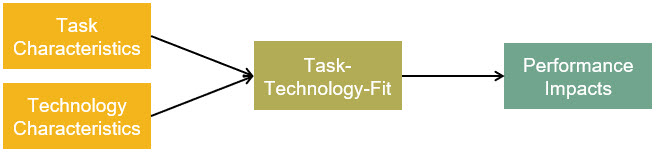
\includegraphics[width=0.8\textwidth]{img/TTF_einfach.jpg}
    \caption[Modell der Task-Technology-Fit Theorie]{Modell der Task-Technology-Fit Theorie\autocite{TTF}}
    \label{fig:TTF}
\end{figure}
\footnotetext{Vgl. eigene Darstellung angeleht an: Spies et al., 2020, S. 399.}
%\footnotetext{Vgl. eigene Darstellung angelehnt an: Goodhue und Thompson, 1995, S. 215.}

\improvement{Abbildung größer und das Balkendiagramm kleiner}

Das \acs{ttf}-Modell kann auf jeder Abstraktionsebene angewendet werden, da die aus der Anforderungsübereinstimmung resultierenden Produktivitätsverbesserungen nicht auf einzelne Personen beschränkt sind und auch für ganze Teams oder komplette Organisationen auftreten können.\autocite[Vgl.][S. 1827f]{GOODHUE1995b} 


%Hierbei kann die TTF-Analyse auf verschiedenen Abstraktionsebenen durchgeführt werden, da die Vorteile der Verbesserung der Produktivität nicht nur auf Einzelpersonen, sondern auch auf ganze Organisationen übertragen werden können.\autocite[Vgl.][S. 1827f]{GOODHUE1995b} Eine verbesserte Leistung kann gemäß TTF auf die reibungslose Ausführung der Aufgabe, die Verringerung der Kosten für die Ausführung der Aufgabe oder die Erleichterung der Aufgabe zurückzuführen. \autocite[Vgl.][S. 96]{LEE2007}

Die Task Charakteristika beziehen sich dabei auf die Gesamtheit der physischen und kognitiven Handlungen und Prozesse, welche von einer Organisation oder einer Einzelperson in einer bestimmten Umgebung ausgeführt werden. Sie werden speziell in Bezug zur Technologie, welche sie bei der Ausführung unterstützen soll, betrachtet und je nach Komplexität auf unterschiedliche Detailebenen heruntergebrochen. \autocite[Vgl.][S. 398]{SPIES2020} Nach Goodhue (1998) können die zur Evaluation der Technologie notwendigen Anforderungen mithilfe eines Task-Modells, einer Literaturrecherche oder mittels Interviews erhoben werden.\autocite[Vgl.][S. 126]{GOODHUE1998} Eine Anforderung wird in diesem Kontext definiert als eine Aussage, \enquote{die einen Bedarf und die damit verbundenen Einschränkungen und Bedingungen darstellt und erläutert}.\autocite[Vgl.][]{ISO2017}

Innerhalb des \acs{ttf}-Modells beziehen sich die Technologie Charakteristika auf die Werkzeuge, welche von Einzelpersonen zur Ausführung ihrer Aufgaben verwendet werden oder diese bei der Ausführung ihrer Aufgaben unterstützen.\autocite[Vgl.][S. 399]{SPIES2020} Dabei kann sowohl der Einfluss eines einzelnen Systems, als auch die Wirkung einer Gesamtheit von bereitgestellten Systemen und Diensten betrachtet werden. \autocite[Vgl.][S. 216]{GOODHUE1995}

%Als Technologie Charakteristiken werden im Rahmen des TTF Modells die Werkzeuge bezeichnet, welche von Einzelpersonen zur Ausführung ihrer Aufgaben oder zur Unterstützung bei der Ausführung ihrer Aufgaben verwendet werden sollen.\autocite[Vgl.][S. 216]{GOODHUE1995} Dabei ist das Modell so allgemein gehalten, dass es sich entweder auf die Einfluss eines bestimmten Systems oder auf die umfassendere Wirkung der Gesamtheit der bereitgestellten Systeme, Strategien und Dienste ausgerichtet sein kann. \autocite[Vgl.][S. 399]{SPIES2020}




\section{Systematische Literaturanalyse}


Im Rahmen des \acs{ttf}-Modells wurde eine systematische Literaturanalyse zur Identifikation der Anforderungen der \ac{kfz}-Versicherer an digitale Plattformen durchgeführt. Hierfür wurden zunächst die für die Task Charakteristika relevanten Suchbegriffe auf Deutsch und Englisch festgelegt, siehe Tabelle \ref{tab:suchbegriffe} im Anhang. Daraufhin wurde mithilfe dieser Suchbegriffe die Datenbanken Google Scholar, EBSCO Discovery Service, \ac{jstor} sowie Google nach Fachliteratur, internationalen und nationalen Zeitschriften, Studien, Magazinen und Internetartikeln durchsucht. Die dabei angewendeten Suchkriterien sind in Tabelle \ref{tab:kriterien} im Anhang aufgezeigt. Grundlage für die Betrachtung der Recherche-Ergebnisse waren der Titel, die Kurzfassung, die Gliederung, die Einleitung sowie die Zusammenfassung der jeweiligen Quelle. Dabei wurden die ausgewählte Literatur zur Identifikation der Task Charakteristika als Ganzes oder in Ausschnitten gelesen und analysiert. \autocite[Vgl.][]{SOLIS2021}

\improvement{Optional: Quelle austauschen}




\section{Semistrukturiertes Leitfadeninterview und qualitative Inhaltsanalyse}

Im Rahmen des \ac{ttf}-Modells werden in dieser Abhandlung zur Validierung, Erweiterung und Priorisierung der in Literatur gefundenen Task-Charakteristika Experteninterviews als qualitative Forschungsmethode eingesetzt. Die Methode ermöglicht das Erschließen bisher unbekannter Aspekte sowie das induktive Erarbeiten von Schlussfolgerungen. Experteninterviews eignen sich insbesondere für explorative Fragestellungen, da sie helfen, das Forschungsfeld zu strukturieren und zu präzisieren. Als Experten können diejenigen Personen betrachtet werden, die durch ihre Funktion oder Tätigkeit spezielles Sonderwissen erwerben konnten. \autocite[Vgl.][S. 119-127]{MISOCH2019} Die Wahl der Experten ist dem Anhang \ref{sec:Expertenwahl} zu entnehmen.

Um ein Experteninterview systematisch zu strukturieren, wird im Voraus vom Interviewer ein Leitfaden, bestehend aus geschlossenen und offenen Fragen sowie optional auch Stichpunkten ausgearbeitet und den Experten zur Verfügung gestellt \autocite[Vgl.][S. 670]{HELFFERICH2019}. Die Kombination von offenen und geschlossenen Fragen ermöglicht es, zum einen ein umfassendes Bild über die Ansichten des Experten zu gewinnen und zum anderen quantitative Aussagen zu erheben, die mit anderen Expertenmeinungen verglichen werden können. Der in der Arbeit verwendete Leitfaden ist thematisch strukturiert, halbstandardisiert, nach den Grundprinzipien von Misoch in vier Phasen untergliedert und im Anhang unter \ref{sec:Fragenkatalog} zu finden \autocite[Vgl.][S. 68f]{MISOCH2019}.  

Für die Auswertung der erhobenen Daten wird die qualitative Inhaltsanalyse nach Mayring verwendet, bei der ein Kategoriensystem deduktiv aus der Literatur und induktiv aus den Antworten der Experten definiert wird \autocite[Vgl.][S. 633-634]{MAYRING2019}. Anhand der Kategorien können Aussagen aus den Interviews zusammengeführt werden, um eine Gesamtanalyse aller Interviews durchzuführen \autocite[Vgl.][S. 74]{BOGNER2014}. 



